\appendix

\section{Anhang}
\subsection{Speicherung der Daten in eXist}
\begin{figure}[H]
	\centering
		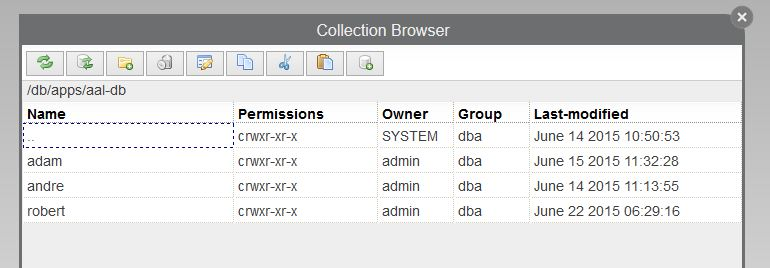
\includegraphics[width=0.8\textwidth]{images/collections1.jpg}
		\caption{Collection für jede Person} 
		\label{collection1}
	\centering
\end{figure}
\begin{figure}[H]
	\centering
		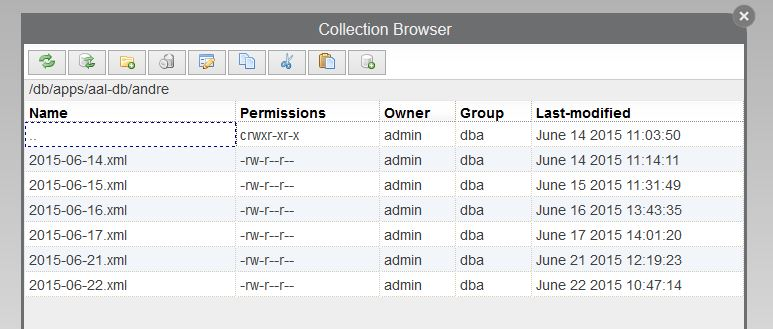
\includegraphics[width=0.8\textwidth]{images/collections2.jpg}
		\caption{XML-Dokument für jeden Tag} 
		\label{collection2}
	\centering
\end{figure}

\subsection{Bedienungsanleitung}
Zunächst muss der Server, auf dem das Projekt gehostet wird, gestartet werden. Dazu öffnet man einen Browser und geht auf die URL \url{http://www.koding.com}. Danach muss man sich bei der Website anmelden. Dazu sind folgende Accountdaten einzugeben:

\begin{itemize}
	\item Email address: aal-xml-projekt@web.de
	\item Password: aalxmlprojekt2014
\end{itemize}

Nach der Anmeldung erscheint eine IDE. Es wird ein Fenster angezeigt, mit der Nachricht, dass die koding-vm-0 offline ist. Klicken Sie auf den Button \textit{"Turn it on"}. Warten Sie 1-2 Minuten, bis die VM hochgefahren ist. Sollte sich beim Fortschritt nichts mehr tun, laden Sie die Seite neu und versuchen Sie erneut die VM hochzufahren.
\\
\\
Ist die VM hochgefahren, wird die IDE komplett sichtbar. Rechts neben der Ordnerstruktur befindet sich das Eingabefenster. Klicken Sie in dem Eingabefenster oben oder unten auf das $+$ und gehen in dem sich öffnenden Kontextmenü auf \textit{New Terminal -> New Session}. In dem sich geöffneten Terminalfenster geben Sie bitte ein: \textit{./serverStart.sh} und betätigen Sie Enter. Nach diesem Schritt ist der Node.JS Server und der eXist gestartet. Bitte lassen Sie das Fenster von Koding.com während der Benutzung der Applikation geöffnet, da es sonst passieren kann, dass die VM heruntergefahren wird.
\\
\\
Danach kann die Seite zur Erzeugung der Sensorwerte unter der URL \url{http://aalxmlprojekt.koding.io/sensor/index.html} geöffnet werden. Zunächst muss hier die \textit{Person ID} und die \textit{Room ID} eingegeben werden (Beispielsweise "wagenknecht"'  und "wohnzimmer"). Danach kann auf den Radio Button neben \textit{Generate normal values} geklickt werden. Hiermit wird die Generierung der Sensorwerte gestartet. Es erscheint ebenfalls darunter eine Tabelle mit den Werten und der Möglichkeit, zu hohe oder zu niedrige Werte erzeugen zu lassen. Im Feld \textit{Change room} kann die \textit{Room ID} geändert werden. Über den Button \textit{Stop} wird die Generierung beendet.
\\
\\
Um den Webclient für das Monitoring zu starten, geht man auf folgende URL: \url{http://aalxmlprojekt.koding.io/client/clientPage.xhtml}. Hier kann man eine \textit{Person ID} im oberen Feld eingeben und mit dem Button bestätigen. In diesem Beispiel könnte die ID "wagenknecht" genutzt werden. Daraufhin erscheinen bei eingeschaltetem Generator die aktuellen Werte in der darunterliegenden Tabelle. Sollte es einen kritischen Wert geben, wird ein Ton abgespielt. Dieser kann über den Button \textit{Ton abschalten} deaktiviert werden. 
\\
\\
Um nun einen Report zu erzeugen, muss zunächst der Zeitraum eingegeben werden. Bitte geben Sie das Datum in der Form YYYY-MM-DD ein. Wenn man nun auf den Button \textit{Report anfordern} klickt, wird der Report erzeugt. Dies kann je nach Umfang mehrere Sekunden dauern. Sobald der Report vorhanden ist, erscheint ein Button \textit{Ihre Daten}. Hinweis: sollte die angegebene \textit{Person ID} nicht vorhanden sein, wird eine visuelle Meldung ausgegeben. Außerdem werden nur Daten angezeigt, wenn vorher der Generator eingeschaltet wurde.

\subsection{Datengenerator GUI}
\begin{figure}[H]
	\begin{center}
		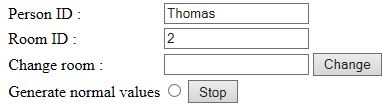
\includegraphics[scale=0.9]{images/eingabe-formular.jpg}
		\caption{Eingabe Formular}
	\end{center}
\end{figure}
\begin{figure}[H]
	\begin{center}
		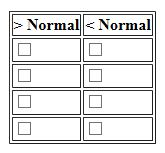
\includegraphics[scale=0.9]{images/kritische-werte-tabelle.jpg}
		\caption{Steuerungsformular}
	\end{center}
\end{figure}
\begin{figure}[H]
	\begin{center}
		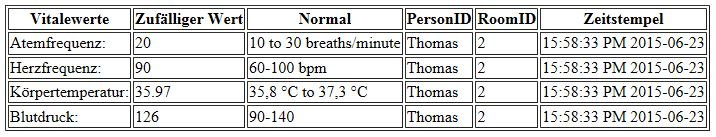
\includegraphics[scale=0.9]{images/vitalwerte-tabelle.jpg}
		\caption{Vitalwerte Tabelle}
	\end{center}
\end{figure}
